\documentclass[a4paper,11pt]{article}
\usepackage{graphicx}
\usepackage[utf8]{inputenc}
\usepackage{hyperref}
\usepackage{placeins}
\usepackage[newfloat]{minted}
\usepackage{caption}

\newenvironment{code}{\captionsetup{type=listing}}{}
\SetupFloatingEnvironment{listing}{name=Code Overview}


\hypersetup{
    colorlinks=true,
    linkcolor=blue,
    filecolor=black,      
    urlcolor=blue,
    citecolor=black,
}
\begin{document}

\title{
    \textbf{Linked List Report.}
}
\author{Adrian Jonsson Sjödin}
\date{Fall 2022}

\maketitle

\section*{Introduction}
The purpose of this assignment is to gain a better understanding of pointers and references
and how they can be used to create more complicated data structures. In particular we will
gain a deeper understanding of how linked lists functions.

\section*{Task}
Implement a linked list class from the ground up that utilizes a stack structure. Also
create a method that allows one to append another linked list to said created linked list.
Having implemented that, benchmark the run time of the append operation. Vary the size of the
first linked list \textbf{a} and append it to a fixed size linked list \textbf{b} and
examine how the run time changes with the size of list \textbf{a}.

Lastly implement the equivalent append operation using arrays and benchmark this operation.
How does this compare to the append operation for the linked list class? Without doing any measurements, 
describe the difference in execution time for this linked list stacked as compared to the stack implemented 
using arrays from the previous assignment.

\section*{Method \& Theory}
I implemented the linked list stack using a private helper class to create nodes that contains the value 
we want to add to the list, and a pointer to the next node in the list. So when a linked list are created 
it is created empty and when we want to add a value to it we create a new node that will then have a pointer
\textit{next} that will be null for the first node. But since every new node will be created and added to the 
left of it in the list, they will have a pointer to the previous node already in the list. Figure 
\ref{fig:linkedListDiagram} shows how this would look like and code overview \ref{code:classStructure} shows the code implementation
of this.

\begin{figure}[h]
    \centering
    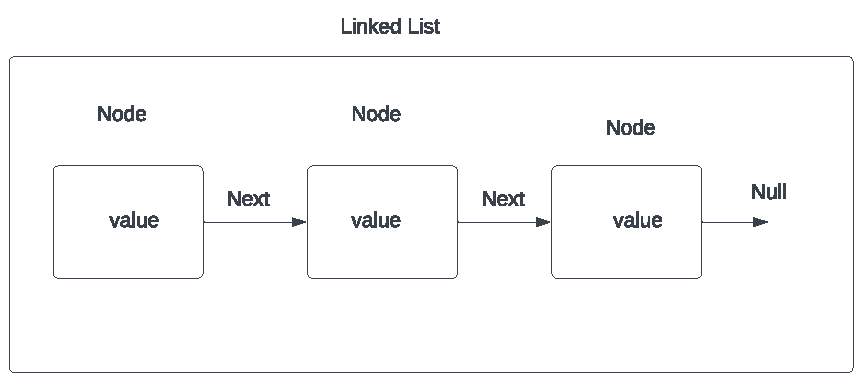
\includegraphics[width=.8\textwidth]{linkedListDiagram.pdf}
    \caption{Depiction of node implementation in a linked list}
    \label{fig:linkedListDiagram}
\end{figure}
When we want to add a new value to the list, the linked list class then only need to keep track of the \textit{head} 
node and rereference it to point at the new node, and make sure that the new node point at the old head node. 
The old node in turn already has a reference to the node before it and thus there's nothing else that needs 
to be done. This operation should take constant time ($\mathcal{O}(1)$) regardless of how big the list already is since we don't 
need to do any kind of operation on the list apart from rereferencing the old head node. The code implementation of this can be seen
in code overview \ref{code:add}.

A push operation was also implemented so that the last inserted value could be removed. It works on the same principle as
the add operation and for those interested a link to the full code will be included at the end of this report.

For the append method that should append one linked list to another, two different methods where created. One where we append
the list to the end of the first list, and one where we instead append it to the front of the first list. In theory appending 
the list \textbf{a} that varies in size to the end of the fixed size list \textbf{b} should have a time complexity of 
$\mathcal{O}(1)$. This since list \textbf{b} is fixed and we simply need to step through that list until we reach the node 
that has a null pointer and rereference it to point to the head of list \textbf{a}.

Appending list \textbf{a} to the beginning of list \textbf{b} however should have a time complexity of $\mathcal{O}(a)$, where $a$ 
is the size of list \textbf{a}. This is because just as in the other append method we need to first step through list \textbf{a}
until we reach the null pointer. We then need to make it point to the head of list \textbf{b} and also move the head pointer for list
\textbf{b} to point to the head of list \textbf{a}. An illustration of this can be seen in figure \ref{fig:append} and the code 
can be seen in code overview \ref{code:append}.

Lastly we implement the equivalent append method for appending two arrays. I implemented this in accordance to the instructions provided
in the assignment. This method should have a time complexity of $\mathcal{O}(a+b)=\mathcal{O}(n)$, where $a$ and $b$ is the size of array 
\textbf{a} and \textbf{b}. This since we need to loop through both arrays and copy each element to a new array big enough to hold 
all elements from both arrays.

\begin{figure}[h]
    \centering
    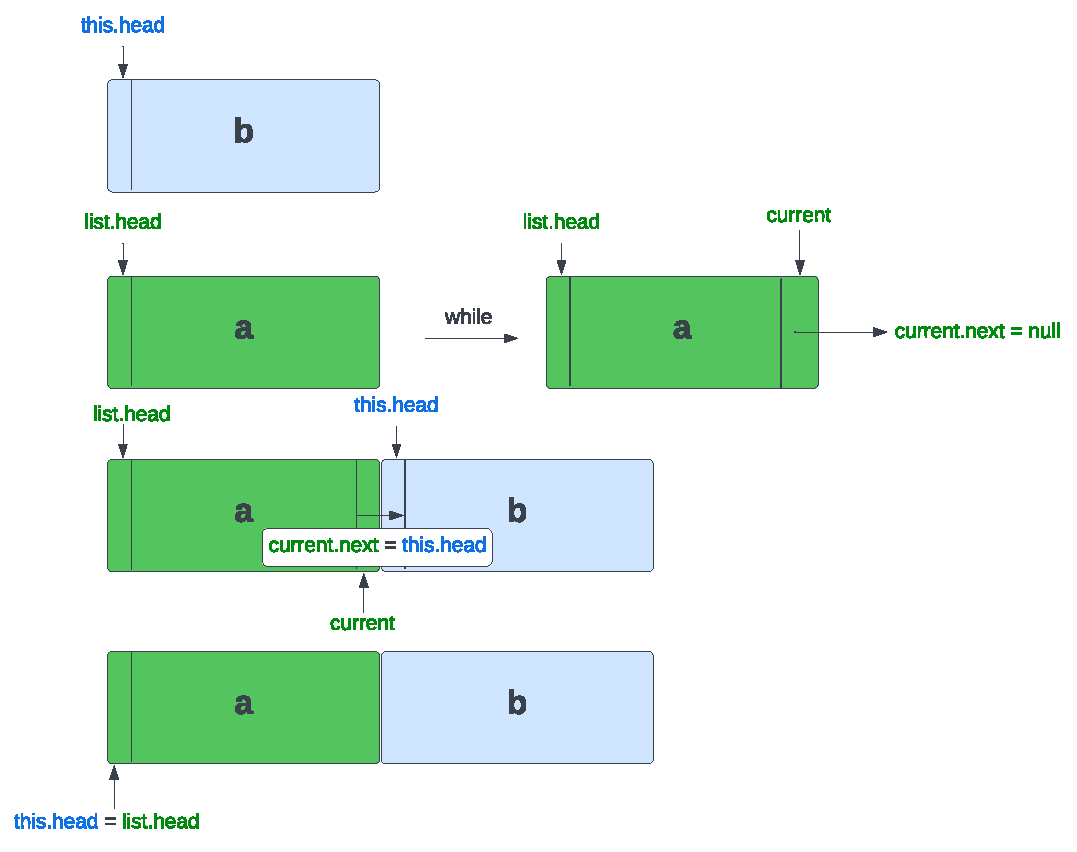
\includegraphics[width=.8\textwidth]{appendDiagram.pdf}
    \caption{Diagram of how the append first method works}
    \label{fig:append}
\end{figure}

\begin{code}
\captionof{listing}{Class Structure}
\label{code:classStructure}
\begin{minted}{java}
public class LinkedList {
    private int size; //track size of list and used to see if list is empty
    private Node head;
    private class Node {
        private int value; // the value for the item we add
        private Node next; // pointer to next element in the list
        public Node(int value, Node node) {
            this.value = value;
            this.next = node;
        }
    }
     public LinkedList() {
        this.size = 0;
        this.head = null;
    }
}
\end{minted}
\end{code}
\newpage
\begin{code}
\captionof{listing}{Add integer to stack}
\label{code:add}
\begin{minted}{java}
 public void add(int value) {
    Node newHead = new Node(value, this.head);
    this.head = newHead;
    this.size++;
 }
\end{minted}
\end{code}

\begin{code}
\captionof{listing}{Append to front of list}
\label{code:append}
\begin{minted}{java}
public void appendFirst(LinkedList linkedList) {
    Node current = linkedList.head;
    while (current.next != null) {
        current = current.next;
    }
    current.next = this.head;
    this.head = linkedList.head;
}
\end{minted}
\end{code}

\FloatBarrier
\section*{Result}
Figure \ref{fig:addOperation} shows the minimum time for one add operation out of a thousand add operations done $10,000$ 
times for each benchmark. On average one add operation took $49.9$ ns.

\begin{figure}[h]
    \centering
    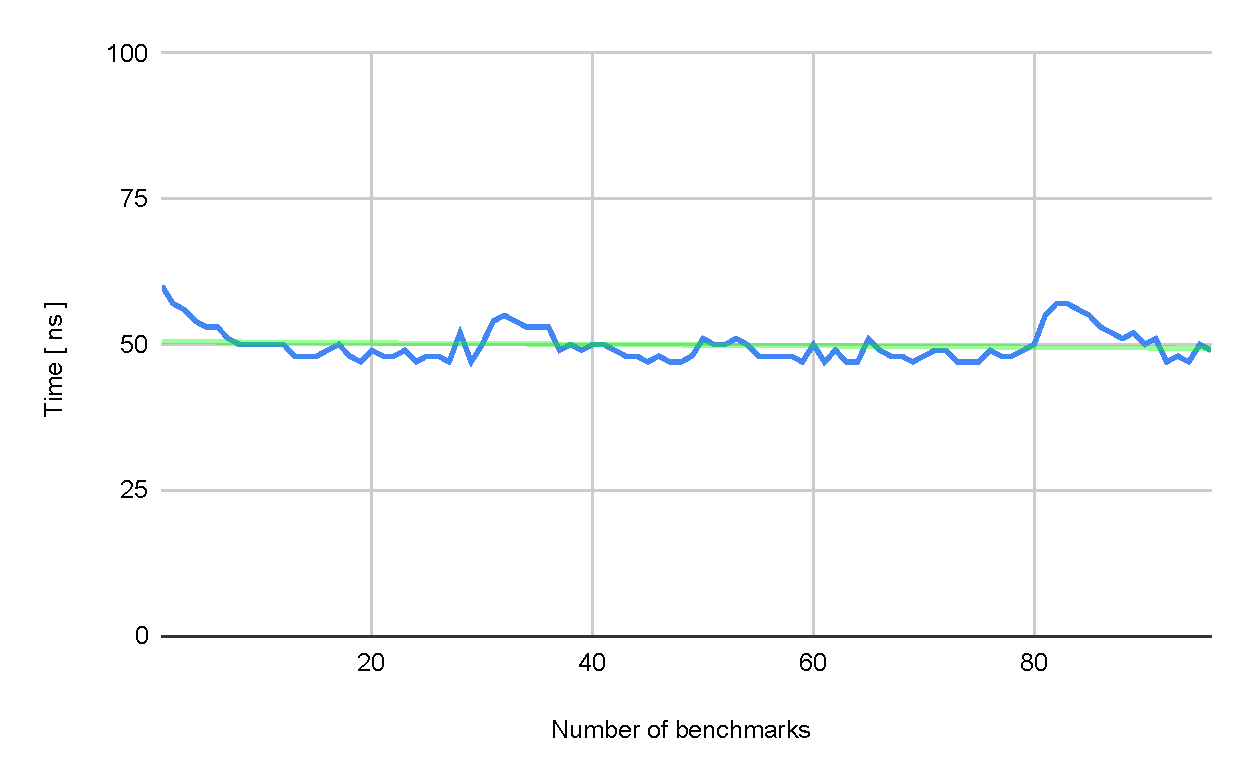
\includegraphics[width=.8\textwidth]{addOperation.pdf}
    \caption{Time for one push operation}
    \label{fig:addOperation}
\end{figure}

Figure \ref{fig:listAppend} shows the benchmark data for appending a growing list to a fixed list. The list increases in size by 
10 for each benchmark up to a size of 1000, and the time is the minimum time from doing this append operation $10,000$ times in 
each benchmark.

\begin{figure}[h]
    \centering
    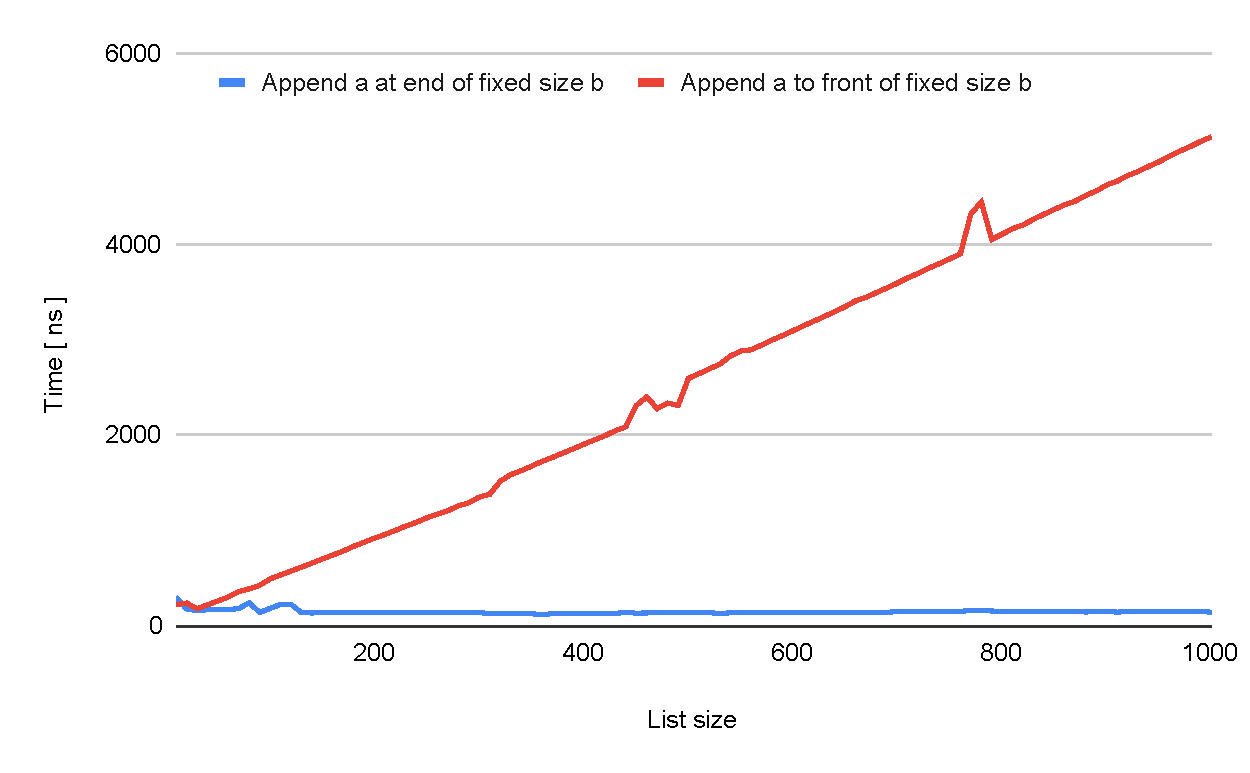
\includegraphics[width=.8\textwidth]{appendList.pdf}
    \caption{Time it takes to append growing list \textbf{a} to fixed size list \textbf{b}}
    \label{fig:listAppend}
\end{figure}

\begin{figure}[h]
    \centering
    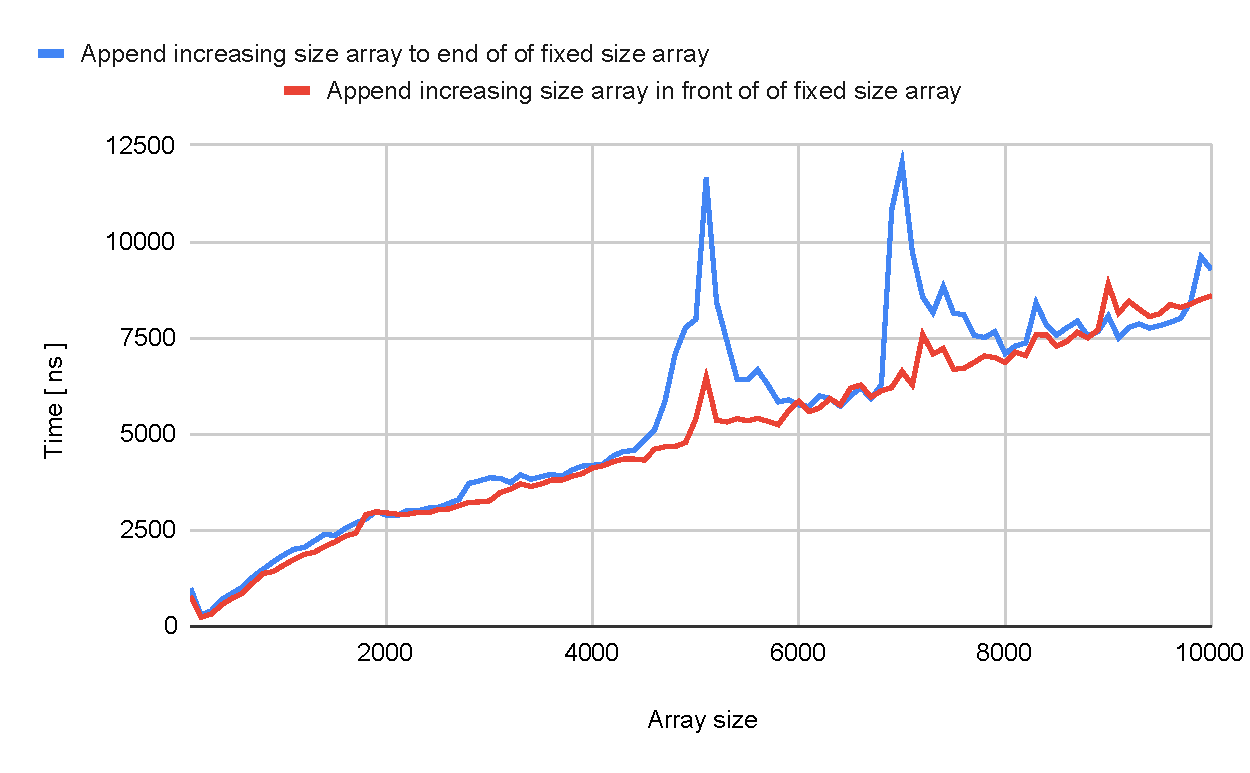
\includegraphics[width=.8\textwidth]{arrayAppend.pdf}
    \caption{Time it takes to append growing array \textbf{a} to fixed array \textbf{b}}
    \label{fig:arrayAppend}
\end{figure}

Figure \ref{fig:arrayAppend} shows the benchmark data for appending a growing array to a fixed size array. The array increases in 
size by 100 for each benchmark up to a size of $10,000$, and the time is the minimum time from doing this append operation $10,000$ 
times. 

In both the benchmark for the list and the array, the benchmark are run on a new unmodified list and array. 
\FloatBarrier
\section*{Discussion}



\end{document}
